% Drawing 154/07-1 -- folder 154, batch 07, archive page 121 (PDF page 122).
% Transcription: page de dessins en couleur, sans texte. En haut, quatre petits rectangles bordés de vert ou de brun, traversés de droites rouges qui se croisent. Un disque bordé de vert, rempli de pseudo-droites rouges, traversé par deux droites vert clair fléchées marquées $D_1$ et $D_\nu$ ; un disque rouge rempli de courbes rouges et vertes qui vont d'un point du bord au point opposé. Au crayon, trois droites $D_2$, $D_0$, $D_1$ qui passent à travers deux croisements orange. Au milieu, une droite vert clair qui contourne des croisements orange, les sommets marqués $s_p$, $s_0$, $s_1$, $s_2$, et les étiquettes $D_p$, $D_1$, $D_\nu$. En bas, un hexagone rouge au pourtour épais, rempli de tirets orange, aux sommets duquel se croisent des droites rouges (deux points marqués) ; une grille de droites rouges et orange ; une bande de droites vert clair coupée de croisements orange, avec un chemin en tirets
% Kind: page of colour drawings: rectangles, disks with arrangements, lines round crossings, hexagon, grid. Method 2 (schematic redraw from the facsimile). Status: partial.
% Notes: Page of colour drawings without text, over a printed dataset table (not reproduced), read from the page view. Top: four small rectangles bordered in green or brown, crossed by red lines that cross. A disk bordered in green, filled with red pseudolines, crossed by two arrowed light green lines D_1 and D_nu; a red disk filled with red and green curves from a point of the rim to the opposite point. In pencil, three lines D_2, D_0, D_1 through two orange crossings. In the middle, a light green line going round orange crossings, vertices s_p, s_0, s_1, s_2 and labels D_p, D_1, D_nu (vertex labels not reproduced). Bottom: a red hexagon with a thick outline filled with orange dashes, red lines crossing at its vertices (two points marked); a grid of red and orange lines; a band of light green lines cut by orange crossings with a dashed path. Arrangements schematic; pencil ovals in the middle left out.
% Coordinates: 1 unit = 1 mm = 1/100 of the crop width (bbox in page fractions: [0.148, 0.085, 0.964, 0.528]).
% Redrawn by Claude (claude-opus-5-5), issue #73, 2026-11-07; not checked by a human; not compiled (no TeX in the session).
% Rights: reproduces part of the work -- behind RENDER_TRANSCRIPTS, never published by itself.
\documentclass[tikz,border=3pt]{standalone}
\usepackage{amsmath,amssymb}
\usetikzlibrary{patterns,arrows.meta}
\tikzset{Or/.style={orange!90!black}, Ye/.style={yellow!80!orange}, Lg/.style={green!60!black!70}, Dg/.style={green!45!black}, Br/.style={brown!80!black}, Rd/.style={red!85!black}, Bl/.style={blue!70!black}, Gy/.style={black!40}, pencil/.style={black!45}, struck/.style={black!35}, mark/.style={circle,draw,inner sep=1.3pt}, pt/.style={circle,fill,inner sep=0.9pt}, opt/.style={circle,draw,fill=white,inner sep=1.1pt}}
\begin{document}
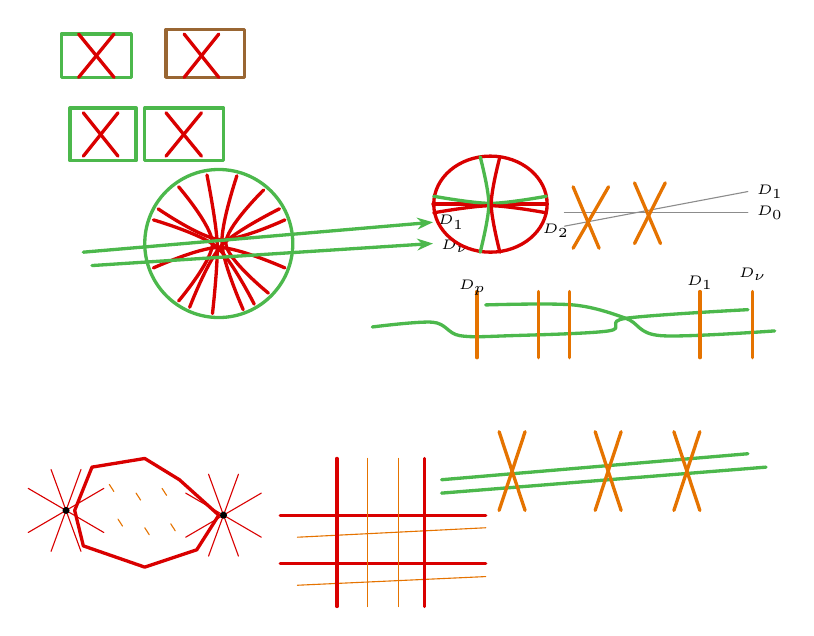
\begin{tikzpicture}[x=1mm,y=1mm,line cap=round,line join=round,font=\scriptsize]
\draw[Lg,very thick] (6.1,-1.7) -- (15,-1.7) -- (15,-7.2) -- (6.1,-7.2) -- cycle;
\draw[Br,very thick] (19.4,-1.1) -- (29.4,-1.1) -- (29.4,-7.2) -- (19.4,-7.2) -- cycle;
\draw[Lg,very thick] (7.2,-11.1) -- (15.6,-11.1) -- (15.6,-17.8) -- (7.2,-17.8) -- cycle;
\draw[Lg,very thick] (16.7,-11.1) -- (26.7,-11.1) -- (26.7,-17.8) -- (16.7,-17.8) -- cycle;
\draw[Rd,very thick] (8.3,-1.7) -- (12.8,-7.2);
\draw[Rd,very thick] (12.8,-1.7) -- (8.3,-7.2);
\draw[Rd,very thick] (21.7,-1.7) -- (26.1,-7.2);
\draw[Rd,very thick] (26.1,-1.7) -- (21.7,-7.2);
\draw[Rd,very thick] (8.9,-11.7) -- (13.3,-17.2);
\draw[Rd,very thick] (13.3,-11.7) -- (8.9,-17.2);
\draw[Rd,very thick] (19.4,-11.7) -- (23.9,-17.2);
\draw[Rd,very thick] (23.9,-11.7) -- (19.4,-17.2);
\draw[Lg,very thick] (26.1,-28.3) ellipse[x radius=9.4, y radius=9.4];
\draw[Rd,very thick] plot[smooth, tension=0.55] coordinates {(24.6,-19.6) (25.9,-28.3) (25.3,-37.2)};
\draw[Rd,very thick] plot[smooth, tension=0.55] coordinates {(28.4,-19.7) (26.5,-28.3) (29.2,-36.7)};
\draw[Rd,very thick] plot[smooth, tension=0.55] coordinates {(21,-21.1) (25.3,-28.3) (21,-35.6)};
\draw[Rd,very thick] plot[smooth, tension=0.55] coordinates {(31.8,-21.5) (27,-28.3) (32.4,-34.6)};
\draw[Rd,very thick] plot[smooth, tension=0.55] coordinates {(18.4,-23.9) (26.2,-27.8) (34.5,-25.3)};
\draw[Rd,very thick] plot[smooth, tension=0.55] coordinates {(17.8,-31.4) (26.1,-28.8) (34.5,-31.4)};
\draw[Rd,very thick] plot[smooth, tension=0.55] coordinates {(33.8,-23.9) (26.4,-28.6) (22.4,-36.4)};
\draw[Rd,very thick] plot[smooth, tension=0.55] coordinates {(17.8,-25.3) (25.8,-28.7) (30.6,-36)};
\draw[Lg,very thick,-{Stealth[length=2mm]}] (8.9,-29.4) -- (53.3,-25.6);
\draw[Lg,very thick,-{Stealth[length=2mm]}] (10,-31.1) -- (53.3,-28.3);
\node[inner sep=1pt] at (55.6,-25.6) {\tiny $D_1$};
\node[inner sep=1pt] at (56.1,-28.7) {\tiny $D_\nu$};
\draw[Rd,very thick] (60.6,-23.3) ellipse[x radius=7.2, y radius=6.1];
\draw[Rd,very thick] plot[smooth, tension=0.55] coordinates {(53.3,-23.3) (60.6,-23.3) (67.8,-23.3)};
\draw[Lg,very thick] plot[smooth, tension=0.55] coordinates {(53.4,-22.3) (60.6,-23.2) (67.7,-22.3)};
\draw[Rd,very thick] plot[smooth, tension=0.55] coordinates {(53.4,-24.4) (60.6,-23.5) (67.7,-24.4)};
\draw[Lg,very thick] plot[smooth, tension=0.55] coordinates {(59.3,-17.3) (60.4,-23.3) (59.3,-29.4)};
\draw[Rd,very thick] plot[smooth, tension=0.55] coordinates {(61.8,-17.3) (60.7,-23.3) (61.8,-29.4)};
\draw[pencil] (70,-26.1) -- (93.3,-21.7);
\draw[pencil] (70,-24.4) -- (93.3,-24.4);
\draw[Or,very thick] (71.1,-21.1) -- (74.4,-28.9);
\draw[Or,very thick] (75.6,-21.1) -- (71.1,-28.9);
\draw[Or,very thick] (78.9,-20.6) -- (82.2,-28.3);
\draw[Or,very thick] (82.8,-20.6) -- (78.9,-28.3);
\node[inner sep=1pt] at (96.1,-21.7) {\tiny $D_1$};
\node[inner sep=1pt] at (96.1,-24.4) {\tiny $D_0$};
\node[inner sep=1pt] at (68.9,-26.7) {\tiny $D_2$};
\draw[Lg,very thick] plot[smooth, tension=0.55] coordinates {(45.6,-38.9) (53.3,-38.3) (56.7,-40) (63.3,-40) (75.6,-39.4) (77.8,-37.8) (93.3,-36.7)};
\draw[Lg,very thick] plot[smooth, tension=0.55] coordinates {(60,-36.1) (71.1,-36.1) (77.8,-37.8) (82.2,-40) (96.7,-39.4)};
\draw[Or,very thick] (58.9,-34.4) -- (58.9,-42.8);
\draw[Or,very thick] (66.7,-34.4) -- (66.7,-42.8);
\draw[Or,very thick] (70.6,-34.4) -- (70.6,-42.8);
\draw[Or,very thick] (87.2,-34.4) -- (87.2,-42.8);
\draw[Or,very thick] (93.9,-34.4) -- (93.9,-42.8);
\node[inner sep=1pt] at (58.3,-33.9) {\tiny $D_p$};
\node[inner sep=1pt] at (87.2,-33.3) {\tiny $D_1$};
\node[inner sep=1pt] at (93.9,-32.2) {\tiny $D_\nu$};
\draw[Rd,very thick] (7.8,-62.2) -- (10,-56.7) -- (16.7,-55.6) -- (21.1,-58.3) -- (26.1,-62.8) -- (23.3,-67.2) -- (16.7,-69.4) -- (8.9,-66.7) -- cycle;
\draw[Rd] (1.9,-65) -- (11.5,-59.4);
\draw[Rd] (4.8,-67.4) -- (8.6,-57);
\draw[Rd] (8.6,-67.4) -- (4.8,-57);
\draw[Rd] (11.5,-65) -- (1.9,-59.4);
\draw[Rd] (21.9,-65.6) -- (31.5,-60);
\draw[Rd] (24.8,-68) -- (28.6,-57.6);
\draw[Rd] (28.6,-68) -- (24.8,-57.6);
\draw[Rd] (31.5,-65.6) -- (21.9,-60);
\draw[Or,dashed] (12.2,-58.9) -- (13.3,-60.6);
\draw[Or,dashed] (15.6,-60) -- (16.7,-61.7);
\draw[Or,dashed] (18.9,-59.4) -- (20,-61.1);
\draw[Or,dashed] (13.3,-63.3) -- (14.4,-65);
\draw[Or,dashed] (16.7,-64.4) -- (17.8,-66.1);
\draw[Or,dashed] (20,-63.9) -- (21.1,-65.6);
\node[pt] at (6.7,-62.2) {};
\node[pt] at (26.7,-62.8) {};
\draw[Rd,very thick] (33.9,-62.8) -- (60,-62.8);
\draw[Rd,very thick] (33.9,-68.9) -- (60,-68.9);
\draw[Or] (36.1,-65.6) -- (60,-64.4);
\draw[Or] (36.1,-71.7) -- (60,-70.6);
\draw[Rd,very thick] (41.1,-55.6) -- (41.1,-74.4);
\draw[Rd,very thick] (52.2,-55.6) -- (52.2,-74.4);
\draw[Or] (45,-55.6) -- (45,-74.4);
\draw[Or] (48.9,-55.6) -- (48.9,-74.4);
\draw[Lg,very thick] (54.4,-58.3) -- (93.3,-55);
\draw[Lg,very thick] (54.4,-60) -- (95.6,-56.7);
\draw[Lg,dashed] (63.3,-59.4) -- (80,-57.8);
\draw[Or,very thick] (61.7,-52.2) -- (65,-62.2);
\draw[Or,very thick] (65,-52.2) -- (61.7,-62.2);
\draw[Or,very thick] (73.9,-52.2) -- (77.2,-62.2);
\draw[Or,very thick] (77.2,-52.2) -- (73.9,-62.2);
\draw[Or,very thick] (83.9,-52.2) -- (87.2,-62.2);
\draw[Or,very thick] (87.2,-52.2) -- (83.9,-62.2);
\end{tikzpicture}
\end{document}
